\documentclass[a4paper]{article}
%\usepackage[a4paper]{geometry}
\usepackage[utf8]{inputenc}

\usepackage{amsmath,amsfonts,amssymb,amsthm}
\usepackage{thmtools}
\usepackage{stmaryrd}
\usepackage{natbib}
\usepackage{url}
\usepackage{array}
\usepackage{arydshln}
\usepackage{ifthen}
\usepackage{ifpdf}
\usepackage{verbatim}
\usepackage{mathpartir}

\usepackage{rotating}

\usepackage{mathtools}
\DeclarePairedDelimiter\ceil{\lceil}{\rceil}
\DeclarePairedDelimiter\floor{\lfloor}{\rfloor}

\usepackage{appendix}

\usepackage{tikz}
\usepackage{multirow,bigdelim}

%% make latex preview-mode work with natbib...
\usepackage[displaymath,floats,graphics,textmath,footnotes]{preview}

\declaretheorem[numbered=yes,name=Lemma,qed=$\blacksquare$]{lemma}
\declaretheorem[numbered=yes,name=Definition,qed=$\blacksquare$]{definition}
\declaretheorem[numbered=yes,name=Specification,qed=$\blacksquare$]{specification}

\newcommand{\forcenewline}{$\phantom{v}$\\}
\newcommand{\judgment}[2]{\paragraph{#1}\hspace{\stretch{1}}\fbox{$#2$}}

\newcommand{\update}[2]{[#1 \mapsto #2]}
\newcommand{\sem}[1]{\left\llbracket #1 \right\rrbracket}

%Math notation
\newcommand{\restrictfun}[1]{|_{#1}}
\newcommand{\parfun}{\rightharpoonup}
\newcommand{\finparfun}{\xrightharpoonup{\textit{\tiny{fin}}}}
\newcommand{\monnefun}{\xrightarrow{\textit{\tiny{mon, ne}}}}
\newcommand{\monfun}{\xrightarrow{\textit{\tiny{mon}}}}
\newcommand{\nefun}{\xrightarrow{\textit{\tiny{ne}}}}
\newcommand{\fun}{\rightarrow}
\newcommand{\defeq}{\stackrel{\textit{\tiny{def}}}{=}}
\newcommand{\nequal}[1][n]{\stackrel{\tiny{#1}}{=}}
\newcommand{\nsubeq}[1][n]{\stackrel{\tiny{#1}}{\subseteq}}
\newcommand{\nsupeq}[1][n]{\stackrel{\tiny{#1}}{\supseteq}}
\newcommand{\union}{\mathbin{\cup}}
\DeclareMathOperator{\dom}{dom}
\newcommand{\blater}{\mathop{\blacktriangleright}}
\newcommand{\id}{\var{id}}
\newcommand{\undefined}{\mathit{undefined}}

\newcommand{\powerset}[1]{\mathcal{P}(#1)}

\newcommand{\false}{\mathit{false}}
\newcommand{\true}{\mathit{true}}

%cofes
\newcommand{\cofe}{c.o.f.e.}
\newcommand{\cofes}{\cofe{}'s}
\newcommand{\CatC}{\mathbb{C}}
\newcommand{\CatP}{\mathbb{P}}

%Comments
\newcommand\lau[1]{{\color{purple} \sf \footnotesize {LS: #1}}\\}
\newcommand\dominique[1]{{\color{purple} \sf \footnotesize {DD: #1}}\\}
\newcommand\lars[1]{{\color{purple} \sf \footnotesize {LB: #1}}\\}

%Variables
\newcommand{\var}[1]{\mathit{#1}}
\newcommand{\hs}{\var{ms}}
\newcommand{\ms}{\hs}
\newcommand{\hv}{\var{hv}}
\newcommand{\rv}{\var{rv}}
\newcommand{\lv}{\var{lv}}
\newcommand{\gl}{\var{g}}
\newcommand{\pc}{\mathit{pc}}
\newcommand{\pcreg}{\mathrm{pc}}
\newcommand{\addr}{\var{a}}
\newcommand{\offset}{\var{offset}}
\newcommand{\word}{\var{w}}
\newcommand{\start}{\var{base}}
\newcommand{\addrend}{\var{end}}
\newcommand{\pwlv}{\var{pwl}}
\newcommand{\mem}{\var{mem}}
\newcommand{\reg}{\var{reg}}
\newcommand{\heapseg}{\var{ms}}
\newcommand{\heap}{\var{mem}}
\newcommand{\mode}{\var{mode}}
\newcommand{\perm}{\var{perm}}
\newcommand{\permp}{\var{permPair}}
\newcommand{\roll}{\var{roll}}
\newcommand{\instr}{\var{instr}}
\newcommand{\stdcap}[1][(\perm,\gl)]{\left(#1,\start,\addrend,\addr \right)}
\newcommand{\adv}{\var{adv}}
\newcommand{\msframe}{ms_\var{frame}}
\newcommand{\link}{\var{link}}
\newcommand{\stk}{\var{stk}}
\newcommand{\flag}{\var{flag}}



%Memory projections
\newcommand{\plainproj}[1]{\mathrm{#1}}
\newcommand{\memheap}[1][\Phi]{#1.\plainproj{mem}}
\newcommand{\memreg}[1][\Phi]{#1.\plainproj{reg}}

\newcommand{\updateHeap}[3][\Phi]{#1\update{\plainproj{mem}.#2}{#3}}
\newcommand{\updateReg}[3][\Phi]{#1\update{\plainproj{reg}.#2}{#3}}

%Configuration end states
\newcommand{\failed}{\textsl{failed}}
\newcommand{\halted}{\textsl{halted}}

%Functions
\newcommand{\plainfun}[2]{
  \ifthenelse{\equal{#2}{}}
             {\mathit{#1}}
             {\mathit{#1}(#2)}
}
\newcommand{\decode}{\plainfun{decode}{}}
\newcommand{\encode}{\plainfun{encode}{}}
\newcommand{\encodePerm}{\mathit{encodePerm}}
\newcommand{\encodePermPair}{\plainfun{encodePermPair}{}}
\newcommand{\encodeLoc}{\mathit{encodeLoc}{}}
\newcommand{\decodePermPair}{\plainfun{decodePerm}}
\newcommand{\updatePcPerm}[1]{\plainfun{updatePcPerm}{#1}}

\newcommand{\executeAllowed}[1]{\plainfun{executeAllowed}{#1}}
\newcommand{\nonZero}[1]{\plainfun{nonZero}{#1}}
\newcommand{\readAllowed}[1]{\plainfun{readAllowed}{#1}}
\newcommand{\writeAllowed}[1]{\plainfun{writeAllowed}{#1}}
\newcommand{\withinBounds}[1]{\plainfun{withinBounds}{#1}}
\newcommand{\stdUpdatePc}[1]{\plainfun{updatePc}{#1}}

\newcommand{\readCond}[1]{\plainfun{readCondition}{#1}}
\newcommand{\writeCond}[1]{\plainfun{writeCondition}{#1}}
\newcommand{\execCond}[1]{\plainfun{executeCondition}{#1}}
\newcommand{\entryCond}[1]{\plainfun{entryCondition}{#1}}

\newcommand{\revokeTemp}[1]{\plainfun{revokeTemp}{#1}}
\newcommand{\erase}[2]{\floor*{#1}_{\{#2\}}}


%World operations
\newcommand{\future}{\mathbin{\sqsupseteq}}
\newcommand{\futurewk}{\mathbin{\sqsupseteq}^{\var{pub}}}
\newcommand{\futurestr}{\mathbin{\sqsupseteq}^{\var{priv}}}
\newcommand{\heapSat}[3][\heap]{#1 :_{#2} #3}

\newcommand{\monwknefun}{\xrightarrow[\text{\tiny{$\futurewk$}}]{\textit{\tiny{mon, ne}}}}
\newcommand{\monstrnefun}{\xrightarrow[\text{\tiny{$\futurestr$}}]{\textit{\tiny{mon, ne}}}}


%Assembly labels
\newcommand{\codelabel}[1]{\mathit{#1}}
\newcommand{\init}{\codelabel{init}}
\newcommand{\malloc}{\codelabel{malloc}}
\newcommand{\counter}{\codelabel{counter}}
\newcommand{\iocap}{\codelabel{iocap}}

%Type(s)
\newcommand{\type}[1]{\mathrm{#1}}
\newcommand{\asmType}{\plaindom{AsmType}}


%Domains
\newcommand{\plaindom}[1]{\mathrm{#1}}
\newcommand{\Caps}{\plaindom{Cap}}
\newcommand{\Words}{\plaindom{Word}}
\newcommand{\Addrs}{\plaindom{Addr}}
\newcommand{\ExecConfs}{\plaindom{ExecConf}}
\newcommand{\RegName}{\plaindom{RegisterName}}
\newcommand{\Regs}{\plaindom{Reg}}
\newcommand{\Heaps}{\plaindom{Mem}}
\newcommand{\HeapSegments}{\plaindom{MemSegment}}
\newcommand{\Confs}{\plaindom{Conf}}
\newcommand{\Instrs}{\plaindom{Instructions}}
\newcommand{\nats}{\mathbb{N}}
\newcommand{\ints}{\mathbb{Z}}
\newcommand{\Perms}{\plaindom{Perm}}
\newcommand{\Globals}{\plaindom{Global}}

\newcommand{\Rel}{\plaindom{Rel}}
\newcommand{\States}{\plaindom{State}}
\newcommand{\RegionNames}{\plaindom{RegionName}}
\newcommand{\Regions}{\plaindom{Region}}
\newcommand{\Reg}{\plaindom{Reg}}
\newcommand{\Worlds}{\plaindom{World}}
\newcommand{\Wor}{\plaindom{Wor}}
\newcommand{\Worwk}{\Wor_{\futurewk}}
\newcommand{\Worstr}{\Wor_{\futurestr}}
\newcommand{\xiwk}{\xi_{\var{wk}}}
\newcommand{\xistr}{\xi_{\var{str}}}
\newcommand{\StorePred}{\plaindom{MemSegPred}}
\newcommand{\UPred}[1]{\plaindom{UPred}(#1)}
\newcommand{\DCPred}[1]{\plaindom{P}^\downarrow(#1)}

\newcommand{\Views}{\plaindom{View}}

%LR
\newcommand{\intr}[2]{\mathcal{#1}}
\newcommand{\valueintr}[1]{\intr{V}{#1}}
\newcommand{\exprintr}[1]{\intr{E}{#1}}
\newcommand{\contintr}[1]{\intr{K}{#1}}
\newcommand{\regintr}[1]{\intr{R}{#1}}
\newcommand{\stdvr}{\valueintr{\asmType}}
\newcommand{\stder}{\exprintr{\asmType}}
\newcommand{\stdrr}{\regintr{\asmType}}
\newcommand{\stdkr}{\contintr{\asmType}}
\newcommand{\observations}{\mathcal{O}}
\newcommand{\npair}[2][n]{\left(#1,#2 \right)}

%Reference register/memory
\newcommand{\refreg}[1]{\lfloor #1 \rfloor}
\newcommand{\refheap}[1]{\langle #1 \rangle_m}

%Instructions
%No arguments
\newcommand{\zinstr}[1]{\mathtt{#1}}
\newcommand{\fail}{\zinstr{fail}}
\newcommand{\halt}{\zinstr{halt}}
%One argument
\newcommand{\oneinstr}[2]{\zinstr{#1} \; #2}
\newcommand{\jmp}[1]{\oneinstr{jmp}{#1}}
%Two arguments
\newcommand{\twoinstr}[3]{\zinstr{#1} \; #2 \; #3}
\newcommand{\restricttwo}[2]{\twoinstr{restrict}{#1}{#2}}
\newcommand{\jnz}[2]{\twoinstr{jnz}{#1}{#2}}
\newcommand{\isptr}[2]{\twoinstr{isptr}{#1}{#2}}
\newcommand{\geta}[2]{\twoinstr{geta}{#1}{#2}}
\newcommand{\getb}[2]{\twoinstr{getb}{#1}{#2}}
\newcommand{\gete}[2]{\twoinstr{gete}{#1}{#2}}
\newcommand{\getp}[2]{\twoinstr{getp}{#1}{#2}}
\newcommand{\getl}[2]{\twoinstr{getl}{#1}{#2}}
\newcommand{\move}[2]{\twoinstr{move}{#1}{#2}}
\newcommand{\store}[2]{\twoinstr{store}{#1}{#2}}
\newcommand{\load}[2]{\twoinstr{load}{#1}{#2}}
\newcommand{\lea}[2]{\twoinstr{lea}{#1}{#2}}
%Three arguments
\newcommand{\threeinstr}[4]{\zinstr{#1} \; #2 \; #3 \; #4}
\newcommand{\restrict}[3]{\threeinstr{restrict}{#1}{#2}{#3}}
\newcommand{\subseg}[3]{\threeinstr{subseg}{#1}{#2}{#3}}
\newcommand{\plus}[3]{\threeinstr{plus}{#1}{#2}{#3}}

%Permissions
\newcommand{\plainperm}[1]{\mathrm{#1}}
\newcommand{\noperm}{\plainperm{o}}
\newcommand{\readonly}{\plainperm{ro}}
\newcommand{\readwrite}{\plainperm{rw}}
\newcommand{\exec}{\plainperm{rx}}
\newcommand{\entry}{\plainperm{e}}
\newcommand{\rwx}{\plainperm{rwx}}
%PWL permissions
\newcommand{\readwritel}{\plainperm{rwl}}
\newcommand{\rwlx}{\plainperm{rwlx}}

%Global/local
\newcommand{\local}{\plainperm{local}}
\newcommand{\glob}{\plainperm{global}}

\newcommand{\localReg}{\var{localReg}}
\newcommand{\globalReg}{\var{globalReg}}

%Views
\newcommand{\plainview}[1]{\mathrm{#1}}
\newcommand{\perma}{\plainview{perm}}
\newcommand{\temp}{\plainview{temp}}
\newcommand{\revoked}{\plainview{revoked}}

%OP sem
\newcommand{\diverge}[1][n]{\not\Downarrow_{#1}}
\newcommand{\step}[1][]{\rightarrow_{#1}}

\begin{document}
\begin{flushright}
\today
\end{flushright}
\section{Domains and Notation}
\begin{align*}
\Addrs &::= \nats\\
\Words &::= \Caps + \ints \\
\Regs  &::= \RegName \rightarrow \Words\\
\Heaps &::= \Addrs \rightarrow \Words \\
\Perms &::= \{ \noperm, \readonly, \readwrite, \readwritel, \exec, \entry, \rwx, \rwlx\}\\
\ExecConfs  &::= \Regs \times \Heaps \\
\Caps  &::= (\Perms \times \Globals) \times \Addrs \times (\Addrs + \{ \infty \}) \times \Addrs\\
\Confs &::= \ExecConfs + \{\failed, \halted \times \ExecConfs\} \\
\HeapSegments &::= \Addrs \parfun \Words\\
\Globals & ::= \{\glob, \local \}
\end{align*}
Local capabilities have been added by adding a new domain $\Globals$ which represents whether a capability is local or global. Two new permissions $\readwritel$ and $\rwlx$ that permits writing local capabilities. They are otherwise the same as their non-''permit write local'' counterparts.

The $\glob$ and $\local$ are ordered as shown in Figure~\ref{fig:glob-hier}.
\begin{figure}[!h]
  \centering
  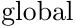
\begin{tikzpicture}[main node/.style={}]
  \node[main node] (1) {$\glob$};
  \node[main node] (2) [below of=1] {$\local$};

  \path[every node/.style={font=\sffamily\small}]
    (1) edge (2);
\end{tikzpicture}
\caption{Permission hierarchy}
\label{fig:glob-hier}
\end{figure}

Things to note:
\begin{itemize}
\item $\RegName$ contains $\pcreg$, but is otherwise a sufficiently
  large finite set.
\item Table~\ref{tab:permission-list} describes what all the permissions grant access to.
\item Figure~\ref{fig:perm-hier} shows the ordering of the permissions, i.e, the elements of $\Perms$.
\item Figure~\ref{fig:glob-hier} shows the ordering of $\local$ and $\glob$, i.e., the elements of $\Globals$.
\item The ordering of $\Perms \times \Globals$ is point wise.
\end{itemize}

\begin{table}[!h]
  \centering
  \begin{tabular}[!h]{r |  p{7cm} }
  $\noperm$ & No permissions. Grants no permissions\\
\hline
  $\readonly$ & Read only. Grants read permission \\
\hline
  $\readwrite$ & Read-write. Grants read and write permissions. Storage of local capabilities prohibited. \\
\hline
  $\readwritel$ & read-write, permit write local. Grants read and write permissions. Storage of local capabilities granted. \\
\hline
  $\exec$ & Execute permission. Grants execute and read permissions.\\
\hline
  $\entry$ & Entry permission. This permission grants no access, but when jumped to, it Will turn into an $\exec$ permission.\\
\hline
  $\rwx$ & Read, write, execute permission. Grants read, write, and execute permissions. Storage of local capabilities prohibited. \\
\hline
  $\rwlx$ & Read, write, execute permission with permit write local. Grants read, write, and execute permissions. Storage of local capabilities possible.
\end{tabular}

\caption{The permissions in this capability system}
\label{tab:permission-list}
\end{table}
\begin{figure}[!h]
  \centering
  \begin{tikzpicture}[main node/.style={}]
    \node[main node] (7) {$\rwlx$};
    \node[main node] (8) [below left of=7] {$\readwritel$};
    \node[main node] (1) [below right of=7] {$\rwx$};
    \node[main node] (2) [below right of=1] {$\exec$};
    \node[main node] (3) [below right of=2] {$\entry$};
    \node[main node] (4) [below left of=1] {$\readwrite$};
    \node[main node] (5) [below right of=4] {$\readonly$};
    \node[main node] (6) [below right of=5] {$\noperm$};

  \path[every node/.style={font=\sffamily\small}]
    (7) edge (8)
    (7) edge (1)
    (8) edge (4)
    (1) edge (2)
    (2) edge (3)
    (2) edge (5)
    (3) edge (6)
    (1) edge (4)
    (4) edge (5)
    (5) edge (6);
\end{tikzpicture}

\caption{Permission hierarchy}
\label{fig:perm-hier}
\end{figure}
Notation:
\[
\begin{array}{rcl}
i       &\in& \Instrs \\
r       &\in& \RegName\\
\pc     &\in& \Caps \\
\pcreg  &\in& \RegName \\
\Phi    &\in& \ExecConfs \\
\memheap&\in& \Heaps \\
\memreg &\in& \Regs \\
\addr   &\in& \Addrs\\
\perm   &\in& \Perms\\
((\perm,\gl),\start,\addrend,\addr) &\in& \Caps \\
n       &\in& \ints\\
\end{array}
\]
Further definitions:
\[
\begin{array}{rcl}
\lv    &::=& \refreg{r} \\
\hv    &::=& \refheap{r}\\
\rv    &::=& n \mid \lv \\
i      &::=& 
             \jmp{\lv} \mid 
             \jnz{\lv}{\rv} \mid
             \move{\lv}{\rv} \mid 
             \load{\lv}{\hv} \mid 
             \store{\hv}{\rv} \mid  \\
       &   & \plus{\lv}{\rv}{\rv} \mid 
             \lea{\lv}{\rv} \mid 
             \restricttwo{\lv}{\rv} \mid 
             \subseg{\lv}{\rv}{\rv} \mid  \\
       &   & \isptr{\lv}{\rv} \mid 
             \getp{\lv}{\lv} \mid 
             \getl{\lv}{\lv} \mid 
             \getb{\lv}{\lv} \mid
             \gete{\lv}{\lv} \mid
             \geta{\lv}{\lv} \mid \\
       &   & \fail \mid
             \halt \mid 
\end{array}
\]
Further define $\reg_0 \in \Regs$ such that
\[
  \forall r \in \RegName \ldotp \reg_0(r) = 0
\]



\subsection*{Semantics}
Assume a $\decode$ function that decodes integer to instructions:
\begin{align*}
\decode &:\Words \fun \Instrs
\end{align*}
Assume an $\encodePerm$, $\encodeLoc$, and $\encodePermPair$ function that encodes a permissions, locality, and permission pair, respectively, as an integer:
\begin{align*}
\encodePerm &: \Perms \fun \ints \\
\encodeLoc &: \Globals \fun \ints \\
\encodePermPair &: (\Perms \times \Globals) \fun \ints \\
\end{align*}
Further, assume an inverse function, $\decodePermPair{}$, that decodes permissions
\[
  \decodePermPair{} : \ints \fun (\Perms \times \Globals)
\]
\begin{align*}
  \Phi & \rightarrow \sem{\decode(\memheap(\addr))}(\Phi) & &                                   
                                                              \arraycolsep=0pt
                                                              \begin{array}{l}
                                                                \text{if $\memreg(\pcreg) = \stdcap$}\\
                                                                \quad\text{and $\start \leq \addr \leq \addrend$}\\
                                                                \quad\text{and $\perm \in \{ \exec,\rwx, \rwlx \}$ }
                                                              \end{array}\\
\Phi & \rightarrow \failed                                 & & \text{otherwise}
\end{align*}

A number of functions and predicates used in the definition of $\sem{-}$ (defined later). Notice all of them are total.
\begin{align*}
  \executeAllowed{\perm} &=
                           \begin{cases}
                             \true & \text{if } \perm \in \{ \rwx, \rwlx, \exec, \entry \} \\
                             \false & \text{otherwise}
                           \end{cases} \\
  \readAllowed{\perm} &=
                           \begin{cases}
                             \true & \text{if } \perm \in \{ \rwx, \rwlx, \exec, \readwrite, \readwritel, \readonly \} \\
                             \false & \text{otherwise}
                           \end{cases} \\
  \writeAllowed{\perm} &=
                           \begin{cases}
                             \true &
                               \text{if } \perm \in \{ \rwx, \rwlx, \readwrite, \readwritel\} \\
                             \false & \text{otherwise}
                           \end{cases} \\
  \updatePcPerm{w} &=
                                     \begin{cases}
                                       ((\exec,\gl),\start,\addrend,\addr) & \text{if $w = ((\entry,\gl),\start,\addrend,\addr)$}\\
                                       w & \text{otherwise} 
                                     \end{cases} \\
  \nonZero{w} &=
                \begin{cases}
                  \true & \text{if $w\in \Caps$ or $w\in \ints$ and $w \neq 0$}\\
                  \false & \text{otherwise}
                \end{cases} \\
  \withinBounds{(\_,\start,\addrend,\addr)} &=
                                              \begin{cases}
                                                \true  & \text{if $\start \leq \addr \leq \addrend$} \\
                                                \false & \text{otherwise}
                                              \end{cases} \\
  \stdUpdatePc{\Phi} &=
                       \begin{cases}
                         \updateReg{\pcreg}{\var{newPc}} & 
                           \arraycolsep=0pt
                           \begin{array}[t]{l}
                             \text{if $\memreg(\pcreg) = \stdcap$}\\
                             \quad\text{and $\var{newPc} = ((\perm,\gl),\start,\addrend,\addr + 1)$}\\
                           \end{array} \\
                           \failed & \text{otherwise}
                       \end{cases} \\
\end{align*}
%TODO: \Phi.reg(rv) to some other notation. It should only look up reg, if it is a regname otherwise just the litteral.
\begin{align*}
  \sem{\fail}(\Phi)                        & = \failed \\
  \sem{\halt}(\Phi)                        & = (\halted,\Phi) \\
  \sem{\jmp{\lv}}(\Phi)                    & = \updateReg{\pcreg}{\updatePcPerm{\memreg(\lv)}} \\
  \sem{\jnz{\lv}{\rv}}(\Phi)               & = 
                                             \begin{cases}
                                               \updateReg{\pcreg}{\updatePcPerm{\memreg(\lv)}} &
                                               \arraycolsep=0pt
                                               \begin{array}[t]{l}
                                                 \text{if $\nonZero{\memreg(\rv)}$} 
                                               \end{array}\\
                                               \stdUpdatePc{\Phi} & \text{if not $\nonZero{\memreg(\rv)}$}\\
                                               \failed & \text{otherwise }
                                             \end{cases} \\
 \sem{\load{\refreg{r_1}}{\refheap{r_2}}}  & = 
                                             \begin{cases}
                                               \stdUpdatePc{\updateReg{r_1}{\var{w}}} &
                                               \arraycolsep=0pt
                                               \begin{array}[t]{l}
                                                 \text{if }\memreg(r_2) = \stdcap = \var{c} \\
                                                 \quad\text{and }\readAllowed{\perm} \text{ and } \withinBounds{\var{c}} \\
                                                 \quad\text{and }\var{w} = \memheap(\addr)
                                               \end{array}\\
                                               \failed & \text{otherwise }
                                             \end{cases}\\
 \sem{\store{\refheap{r_1}}{\refreg{r_2}}} & = 
                                             \begin{cases}
                                               \stdUpdatePc{\updateHeap{\addr}{\var{w}}} &
                                               \arraycolsep=0pt
                                               \begin{array}[t]{l}
                                                 \text{if }\memreg(r_1) = \stdcap = \var{c} \\
                                                 \quad\text{and }\writeAllowed{\perm} \text{ and } \withinBounds{\var{c}} \\
                                                 \quad\text{and }\var{w} = \memreg(r_2)\\
                                                 \quad\text{and if } \var{w} = ((\_,\local),\_,\_,\_) \text{,} \\
                                                 \quad\text{ then } \perm \in \{\rwlx,\readwritel \}
                                               \end{array}\\
                                               \failed & \text{otherwise }
                                             \end{cases}\\
 \sem{\move{\refreg{r_1}}{\rv}}            & = \stdUpdatePc{\updateReg{r_1}{\memreg(\rv)}}
\\
  \sem{\lea{\refreg{r_1}}{\rv}}            & =
                                             \begin{cases}
                                               \stdUpdatePc{\updateReg{r_1}{\var{c}}} &
                                                 \arraycolsep=0pt
                                                 \begin{array}[t]{l}
                                                   \text{if either $n = \rv$ or $\rv = \refreg{r_2}$ and $n = \memreg(r_2)$} \\
                                                   \quad\text{and in either case $n \in \ints $} \\
                                                   \quad\text{and $\memreg(r_1) = \stdcap$}\\
                                                   \quad\text{and $\var{c} = ((\perm,\gl),\start,\addrend,\addr + n)$}
                                                 \end{array}\\
                                               \failed               & \text{otherwise}
                                             \end{cases} 
\\
 % In the M-Machine, lea checks whether the pointer stay within the allowed range in the pointer.
  \sem{\restricttwo{\refreg{r}}{\rv}}           & =
                                             \begin{cases}
                                               \stdUpdatePc{\updateReg{r}{\var{c}}}  &
                                                 \arraycolsep=0pt
                                                 \begin{array}[t]{l}
                                                   \text{if $\memreg(r) = \stdcap[\permp]$}\\
                                                   \quad\text{and either $\rv = n$ or $\memreg(\rv) = n$}\\
                                                   \quad\text{and in either case $n \in \ints$}\\
                                                   \quad\text{and $\var{newPermPair} = \decodePermPair(n)$}\\
                                                   \quad\text{and $\var{newPermPair} \sqsubseteq \permp$}\\
                                                   \quad\text{and $c = (\var{newPermPair},\start,\addrend,\addr)$}
                                                 \end{array}\\
                                               \failed                   & \text{otherwise}
                                             \end{cases} 
\end{align*}
\begin{align*}
  \sem{\plus{\refreg{r_1}}{\rv_1}{\rv_2}}               & =
                                                          \begin{cases}
                                                            \stdUpdatePc{\updateReg{r_1}{n_1+n_2}} &
                                                            \arraycolsep=0pt
                                                            \begin{array}[t]{l}
                                                              \text{if for $i \in \{1,2\}$}\\
                                                              \quad\text{$n_i = \rv_i$ or $n_i = \memreg(\rv_i)$}\\
                                                              \quad\text{and in either case $n_i \in \ints$}
                                                            \end{array}\\
                                                            \failed & \text{otherwise}
                                                          \end{cases}\\
  \sem{\subseg{\refreg{r}}{\rv_1}{\rv_2}} & = 
                                            \begin{cases}
                                              \stdUpdatePc{\updateReg{r}{\var{c}}} &
                                              \arraycolsep=0pt
                                              \begin{array}[t]{l}
                                                \text{if $\memreg{r} = \stdcap[\permp]$} \\
                                                \quad\text{and for $i \in \{1,2\}$}\\
                                                \quad\text{$n_i = \rv_i$ or $n_i = \memreg(\rv_i)$}\\
                                                \quad\text{and in either case $n_i \in \ints$}\\
                                                \quad\text{and $\start \leq n_1 \leq n_2 \leq \addrend$}\\
                                                \quad\text{and $c = (\permp,n_2,n_2,\addr)$}
                                              \end{array} \\
                                              \failed & \text{otherwise}
                                            \end{cases}
 \\
  \sem{\geta{\refreg{r_1}}{\refreg{r_2}}} & = 
                          \begin{cases}
                            \stdUpdatePc{\updateReg{r_1}{\addr}} &
                            \arraycolsep=0pt
                            \begin{array}[t]{l}
                              \text{if $\memreg{r_2} = \stdcap$}
                            \end{array} \\
                            \failed & \text{otherwise}
                          \end{cases}
  \\
  \sem{\getb{\refreg{r_1}}{\refreg{r_2}}} & = 
                          \begin{cases}
                            \stdUpdatePc{\updateReg{r_1}{\start}} &
                            \arraycolsep=0pt
                            \begin{array}[t]{l}
                              \text{if $\memreg{r_2} = \stdcap$}
                            \end{array} \\
                            \failed & \text{otherwise}
                          \end{cases}
  \\
  \sem{\gete{\refreg{r_1}}{\refreg{r_2}}} & = 
                          \begin{cases}
                            \stdUpdatePc{\updateReg{r_1}{\addrend}} &
                            \arraycolsep=0pt
                            \begin{array}[t]{l}
                              \text{if $\memreg{r_2} = \stdcap$}
                            \end{array} \\
                            \failed & \text{otherwise}
                          \end{cases}
  \\
  \sem{\getp{\refreg{r_1}}{\refreg{r_2}}} & = 
                          \begin{cases}
                            \stdUpdatePc{\updateReg{r_1}{\encodePerm(\perm)}} &
                            \arraycolsep=0pt
                            \begin{array}[t]{l}
                              \text{if $\memreg{r_2} = \stdcap$}
                            \end{array} \\
                            \failed & \text{otherwise}
                          \end{cases}
  \\
  \sem{\getl{\refreg{r_1}}{\refreg{r_2}}} & = 
                          \begin{cases}
                            \stdUpdatePc{\updateReg{r_1}{\encodeLoc(\gl)}} &
                            \arraycolsep=0pt
                            \begin{array}[t]{l}
                              \text{if $\memreg{r_2} = \stdcap$}
                            \end{array} \\
                            \failed & \text{otherwise}
                          \end{cases}
  \\
  \sem{\isptr{\refreg{r}}{\rv}} & =  
                          \begin{cases}
                            \stdUpdatePc{\updateReg{r_1}{1}} & \text{if $\memreg{\rv} = \stdcap$} \\
                            \stdUpdatePc{\updateReg{r_1}{0}} & \text{otherwise} 
                          \end{cases}
\end{align*}
\lau{Dominique, apparently there was a reason I had not added the new condition in store to $\writeAllowed{}$. The new condition depends on a case distinction on $w$. It is only if $w$ is a capability that we look into whether it is local or not. But even if $w$ is just an integer, we still need the capability we write through to have some kind of write permission.}

After adding local capabilities, most of the definitions have changed slightly to take into the account new form the capabilities take. The only two instructions that have undergone enough change to deserve to be mentioned are $\store{}$ and $\restrict{}{}{}$. 

$\store{}$ has the same conditions as before, but if what it tries to write is a capability, then it needs to be a write access that permits write local.

$\restrict{}{}{}$ looks like before, but now it uses a ``permission pair'' which is the access permission and whether it is local or not. Whether a $\restrict{}{}{}$ succeeds depends on the ordering, so the real change lies in the new ordering, which is described further above.

Define the following simple macros:

\begin{align*}
  \restrict{r_1}{r_2}{r_3} \; r_4 &\defeq
                                    \begin{aligned}[t]
                                      & \move{r_1}{r_2} \\
                                      & \restrict{r_1}{r_3}{r_4}
                                    \end{aligned} \\
  \subseg{r_1}{r_2}{r_3} \; r_4   &\defeq
                                    \begin{aligned}[t]
                                      & \move{r_1}{r_2} \\
                                      & \subseg{r_1}{r_3}{r_4}
                                    \end{aligned}\\
  \lea{r_1}{r_2} \; r_3           &\defeq
                                    \begin{aligned}[t]
                                      & \move{r_1}{r_2} \\
                                      & \lea{r_1}{r_3}
                                    \end{aligned}\\
  \store{r}{n} &\defeq
                   \begin{aligned}[t]
                     & \move{r_i}{n} \qquad \text{ where $r_i$ unused register}\\
                     & \store{r}{r_i}
                   \end{aligned}
\end{align*}

\section{Malloc specification}
\newcommand{\hsfoot}{\hs_\var{footprint}}
\newcommand{\hsframe}{\hs_\var{frame}}
\newcommand{\size}{\var{size}}
\newcommand{\rio}{r_{io}}
\newcommand{\advb}{\var{adv_{base}}}
\newcommand{\adve}{\var{adv_{end}}}
\newcommand{\initb}{\var{init}_{base}}
\newcommand{\inite}{\var{init}_{end}}
\newcommand{\mrlen}{5cm}
\newcommand{\retm}{\var{ret}_{\malloc}}
\newcommand{\reta}{\var{ret}_{\adv}}
\newcommand{\base}{\var{base}}
\newcommand{\eend}{\var{end}}
\newcommand{\bracket}[1]{\multirow{#1}{*}{\ensuremath{
 \left . \vphantom{\begin{array}{l}
 \ifthenelse{\equal{#1}{1}}{3\\}{
    \ifthenelse{\equal{#1}{2}}{3\\3\\}{
    \ifthenelse{\equal{#1}{3}}{3\\3\\3\\}{
    \ifthenelse{\equal{#1}{4}}{3\\3\\3\\3\\}{
    \ifthenelse{\equal{#1}{5}}{3\\3\\3\\3\\3\\}{
    \ifthenelse{\equal{#1}{6}}{3\\3\\3\\3\\3\\3\\}{
      3\\3\\3\\3\\3\\3\\3\\ %7
  }}}}}}
  \end{array}} \right \}}}
}
\newcommand{\annotate}[2]{\multirow{#1}{\mrlen}{\scriptsize #2}}

\begin{specification}[Malloc v.2]
  $c_\malloc$ satisfies the specification for malloc iff
\[  
  \left\{
  \begin{aligned}
    &\forall \Phi \in \ExecConfs \ldotp \forall m_{\var{footprint}} \in \Heaps\ldotp \hsframe \in \HeapSegments \ldotp \\
    &\quad \forall n, \size \in \nats \ldotp \forall b,e,a \in \Addrs\ldotp\forall p \in \Perms \ldotp \forall W \in \Worlds \ldotp\\
    &\qquad \exists i, \iota_{\malloc,0} \ldotp \\
    &\qquad \quad \forall W \futurewk [i \mapsto \iota_{\malloc,0}] \land \\
    &\qquad \quad \memheap = m_{\var{footprint}} \uplus \hsframe \land\\
    &\qquad \quad \heapSat[m_{\var{footprint}}]{n}{W} \land \\
    &\qquad \quad \memreg(r_1) = \size \land \\
    &\qquad \quad \size \geq 0 \land \\
    &\qquad \quad \memreg(r_0) = (p,b,e,a) \land \\
    &\qquad \quad \memreg(\pcreg) = c_\malloc \\ %and this needs to change with ABI.
    &\qquad \quad \Rightarrow \\
    &\qquad \qquad\exists \Phi' \in \ExecConfs \ldotp \exists m_{\var{footprint}}' \in \Heaps\ldotp \exists \ms_{\var{alloc}} \in \HeapSegments\ldotp\\
    &\qquad \qquad \quad \exists j,k \in \nats \ldotp \exists b',e'\in \Addrs \ldotp \exists W' \in \Worlds \ldotp \\
    &\qquad \qquad \qquad \Phi \step[j]\Phi' \land \\
    &\qquad \qquad \qquad \memheap[\Phi']=m_{\var{footprint}}' \uplus \hs_{\var{alloc}} \uplus \hsframe \land\\
    &\qquad \qquad \qquad W'= W \update{i}{\iota_{\malloc}'} \land W' \futurewk W \land \\
    &\qquad \qquad \qquad \heapSat[m_{\var{footprint}}']{n-j}{W'} \land \\
    &\qquad \qquad \qquad \dom(\hs_{\var{alloc}}) = [b',e'] \land \forall a \in [b',e']\ldotp \hs_{\var{alloc}}(a) = 0  \land \\
    &\qquad \qquad \qquad \memreg[\Phi'] = \memreg[\Phi]\update{\pcreg}{\updatePcPerm{(p,b,e,a)}}\update{r_1}{((\rwx,\glob),b',e',b')} \land \\
    &\qquad \qquad \qquad \size - 1 = e'-b' 
  \end{aligned}\right.
\]
where $\iota_{\malloc,0}$ is the region that initially governs malloc 
\end{specification}
In the specfication above $\iota_\malloc'$ is a future region of the initial region that governs malloc.
\lau{should it be a public or private future world in the premise?}


\section{Macros}
In order to write readable example programs, we provide macros that can be programmed using the instruction set given in the formalisation.
\dominique{how is the return capability constructed: not on the stack, I presume, so  means mallocing a block of memory for the activation record?}
\lau{See the new addition below - when we don't have a stack, then we have no need to ``save'' local capabilities which means that we can have the return code as part of the program. The only thing we have to do is to have the capability point to the return address and make the capability into an entry capability. }
\lau{On further thought, conveniently the examples did not seem to need an activation record, but if we want \texttt{call} to work more generally speaking, then it needs to setup an activation record. I have changed the description of \texttt{call}, so it now uses an activation record. }
\dominique{Similarly: how is malloc invoked?  Do we trust malloc enough to not encapsulate ourselves from it, i.e. provide an rx return capability and use callee-save registers?}
\lau{ I think this is a conceptual question as we can make it work with either. We already trust malloc to give us a fresh piece of memory and not reuse it later on, so we already assume malloc to be somewhat trusted, so why not go all the way? }
\dominique{what does ``fetch the capability ...'' mean?}
\lau{ We don't know where the capability resides, but if it is in memory, then it will be loaded into a register. }
\dominique{Wouldn't it be more clear to provide call with two explicit lists of registers: those which need to be stored, and those which are provided as arguments (i.e. which do not need to be erased)?}
\dominique{Perhaps you could also provide an explicit syntax for ``undefined symbols'' that should be filled in by a linker?}

\subsection{Linking and ABI}
In order to make capabilities to trusted code (and possibly untrusted code) available, we assume that some sort of linker has made these available. This is done in the following way: For every function, the first memory cell the capability for that function governs contains a capability for the list in question. Each function name in a program corresponds to an offset in the table, e.g., \texttt{malloc}. When a name is used in a program, it indicates what entry to pick from the list. The list should always be accessible by taking a copy of the capability in the $\pcreg$-register and adjusting it to point to the first cell it governs.

The capability link list can be shared between multiple functions as it is accessed through a read-only capability.

\subsection{Flag list}
A function may use flags to signal failure. We use the convention that a flag list is available in the second memory cell of a functions code (so just after the linking table). The flag list is accessed through a read-write capability and initially it contains all zero. Like the linking list, each entry is associated with a name which may appear in the macros.

The flag list should never be shared between distrusting parties.

\begin{description}
\item[\texttt{call} $f(\bar{r}_{\var{args}},\bar{r}_{\var{priv}})$] $\bar{r}_{\var{args}}$ and $\bar{r}_{\var{priv}}$ are lists of registers. An overview of this call:
  \begin{itemize}
  \item Set up activation record
  \item Create local enter capability for activation
  \item Clear unused registers
  \item Jump
  \item Upon return: Run activation code
  \end{itemize}
A more detailed description of each of the above steps:
\begin{description}
  \item [Set up activation record]
    \begin{itemize}
    \item Run malloc to get a piece of memory with space for:
    \begin{itemize}
      \item Words in $\bar{r}_{\var{priv}}$
      \item Code return capability (opc)
      \item Activation code
    \end{itemize}
    \item Store the words in $\bar{r}_{\var{priv}}$ to the activation record. 
    \item Adjust the a copy of the current pc to point to the return address and save it to the activation record.
    \item Write the activation code to the activation record.
  \end{itemize}
  \item [Create local enter capability for activation] Make the capability for the activation record point to the beginning of the activation record and restrict it to a local-enter capability. Place this capability in $r_0$.
  \item [Clear unused registers]
    Clear all the register that are not $\pcreg$, $r_0$ or in $\bar{r}_{\var{args}}$.
  \item [Jump] Load the entry $f$ from the linking table to a free register and jump to it.
  \item [Activation code] The activation code does the following:
    \begin{itemize}
    \item Move the stored ``private'' words in to their respective $\bar{r}_{\var{priv}}$ registers.
%    \item Clear all registers but $r_1$, $\pcreg$, and $\bar{r}_{\var{priv}}$.
    \item Load the return address to $\pcreg$
    \end{itemize}
\end{description}
\item[\texttt{malloc $r$ $n$}] Calls malloc to allocates a piece of memory of size $n$. The capability will be stored in register \texttt{r}.

\item[\texttt{assert$_{\var{flag}}$ $r_1$ $r_2$}] Compares the words in register $r_1$ and $r_2$ (if one of them is an integer, then use that in the comparison). If they are equal, then execution continues. If they are unequal, then the assertion flag named $flag$ in the flag list is set to 1 and execution halts (if no flag is specified, then the first flag in the list is set to 1).
\item[cclear $r$] Stores 0 to all the memory cells the capability $r$ governs.\footnote{This may in some cases seem like an unreasonable slow instruction. In a real system it would probably be implemented as a vector operation which allows modification of continous segments of memory rather fast.}
\item[rclear $\bar{r}$] Moves 0 to all the registers in the list $\bar{r}$.
\end{description}
Note:
\begin{itemize}
\item \texttt{call} will fail if we have local capabilities as part of the ``private'' state as it relies on a capability returned by malloc which will not be permit-write-local. Below, we introduce \texttt{scall} which can handle local capabilities in the ``private'' state.
\end{itemize}
\subsection{Stack}
Some programs will assume access to a stack which will be in part indicated by the program macros, but also in the correctness lemma. The stack is accessed through a local $\rwlx$-capability. Programs will assume that the stack resides in some register, say $r_{\var{stk}}$.

The stack will reside entirely in memory. There is no seperation between the memory and the stack, so when we talk about the stack it is as a conceptual thing.

Eventhough the memory is infinite, we will only use a finite part for the stack. If we have allocated too little memory for the stack, and we try to push something anyway, then the execution will fail. As we consider failing admissable, we are okay with this. 

When not in the middle of a push or a pop, the stack capability points to the top word of the stack. For an empty stack, the stack capability points to the address just outside of the range of authority for the stack capability.

\begin{description}
\item[\texttt{push $r$}] Pushes the word in register \texttt{r} to the stack by incrementing the stack capability by one and storing the word through said capability.\footnote{The stack grows upwards.}
\item[\texttt{pop $r$}] Pops the top word of the stack by loading it to register $r$, moves 0 to the address, and decrementing the stack pointer.
\item[\texttt{scall} $f(\bar{r}_{\var{args}},\bar{r}_{\var{priv}})$] $\bar{r}_{\var{args}}$ and $\bar{r}_{\var{priv}}$ are lists of registers. This call assumes $r_{\var{stk}}$ contains a stack capability. An overview of this call:
  \begin{itemize}
  \item Push restore code to the stack.
  \item Push ``private'' registers to the stack.
  \item Push return address capability 
  \item Push stack pointer
  \item Create protected return pointer
  \item Restrict stack capability
  \item Clear unused registers
  \item Jump
  \item Upon return: Run restore code
  \item Return address: Clear the stack segment we gave control over
  \item Restore ``private'' state
  \end{itemize}
A more detailed description of the above steps:
\begin{description}
  \item [Push restore code to the stack]
    Push the restore code to the stack (described later). This code needs to be on the stack to make sure the stack capability can be restored. We try to keep the restore code on the stack minimal.
  \item [Push ``private'' registers to the stack]
    Push all the words in the registers in  $\bar{r}_{\var{priv}}$ to the stack.
  \item [Push return address capability]
    Push a capability for the return address (in the memory) to the stack.
  \item [Push stack pointer]
    Push the full stackpointer to the stack.
  \item [Create protected return pointer]
    Make a new version of the stack pointer that points to the beginning of the restoration code. Restrict it to a local enter-capability and put it in $r_0$. \lau{Do we want to use ``protected return pointer'' to mean a local enter capability?}
  \item [Restrict stack capability]
    Make the stack capability only govern the unused part.
  \item [Clear unused registers]
    Clear all registers but $\pcreg$, $r_0$, $r_{\var{stk}}$, and $\bar{r}_{\var{args}}$.
  \item [Jump] Load the entry $f$ from the linking table to a free register and jump to it.
  \item [Restore code]
    Load the stack capability to $r_{\var{stk}}$. Pop the old program counter to $\pcreg$.
  \item [Return Address:] \forcenewline
    \begin{description}
    \item [Clear the stack segment we gave control over] Store 0 to all the cells the stack capability passed to the callee governed.
    \item [Restore ``private'' state] \forcenewline
      \begin{itemize}
      \item Pop the private state on the stack into their respective $\bar{r}_{\var{priv}}$ registers.
      \item Pop the restore code of the stack
      \end{itemize}
  \end{description}
\end{description}
\item[\texttt{mclear $r$}] Clears all cells $r$ has authority over. 
\end{description}
Note:
\begin{itemize}
\item If we want to have local capabilities as part of our private state, then we need to have a stack and use \texttt{scall}. If we do not have any local capabilities we want to keep around, then we can use \texttt{call}, but it will incur a small memory leak as the activation records cannot be recycled! It is also possible to use a combination of \texttt{scall} and \texttt{call}, but when \texttt{call} is used, then we have no way to store the stack, so we cannot use \texttt{scall} after that.
\item As a rule of thumb: If you have provided an untrusted entity access to part of the stack, then it needs to be cleared upon return.
\item As a rule of thumb: If you receive a stack from an untrusted source, then you need to check that it is a local $\rwlx$-capability and clear it! If any callbacks are provided, then they need to be global.
\item In a real setting due to a limited number of registers, some of the arguments might be spilled to the stack. It would be possible to do something similar here, but to keep
 matters simple, we opt not to do so.
\end{itemize}
\begin{figure}
  \label{fig:stack-before-call}
  \centering
  \begin{tabular}[!h]{r | >{\raggedright\arraybackslash}p{3cm} |}
\multicolumn{2}{l}{Stack} \\
\cline{2-2}
   & \\
   & $\vdots$\\
\cline{2-2}
   & 0 \\
\cline{2-2}
$c_{\var{stk}} \rightarrow$   & local stack\\
   & $\vdots$\\
\cline{2-2}
\end{tabular}
\hspace{1cm}
\begin{tabular}{r | >{\centering\arraybackslash}p{0.75cm} |}
\multicolumn{2}{r}{Register file} \\
\cline{2-2}
$\pcreg$ & $c_{\pc}$\\
\cline{2-2}
$r_0$  & $c_0$ \\
\cline{2-2}
$r_{\var{stk}}$  & $c_{\var{stk}}$ \\
\cline{2-2}
$r_{\var{args},1}$ & $w_{a,1}$ \\
\cline{2-2}
& $\vdots$ \\
\cline{2-2}
$r_{\var{args},n}$ & $w_{a,n}$\\
\cline{2-2}
$r_{\var{priv},1}$ & $w_{p,1}$\\
\cline{2-2}
& $\vdots$ \\
\cline{2-2}
$r_{\var{priv},m}$ & $w_{p,m}$\\
\cline{2-2}
& $\vdots$ \\
\cline{2-2}
\end{tabular}
\caption{This is the first figure of 6 that illustrates how \texttt{scall} works. In this example, the call \texttt{scall $f([r_{\var{args},1},\dots,r_{\var{args},n}],[r_0,r_{\var{priv},1},\dots,r_{\var{priv},m}])$. In this example the two lists of registers are disjoined eventhough that does not have to be the case.}}
\end{figure}


\begin{figure}
  \label{fig:stack-after-push}
  \centering
  \begin{tabular}[!h]{r | >{\raggedright\arraybackslash}p{3cm} |}
\multicolumn{2}{l}{Stack} \\
\cline{2-2}
   & \\
   & $\vdots$\\
\cline{2-2}
$c_{\var{stk}}' \rightarrow$  & $c_{\var{stk}}'$ \\
\cline{2-2}
   & $c_\pc'$ \\
\cline{2-2}
   & $c_0$ \\
\cline{2-2}
   & $w_{p,1}$ \\
\cline{2-2}
   & $\vdots$ \\
\cline{2-2}
   & $w_{p,m}$ \\
\cline{2-2}
   & Restore code \\
\cline{2-2}
   & local stack\\
   & $\vdots$ \\
\cline{2-2}
\end{tabular}
\hspace{1cm}
\begin{tabular}{r | >{\centering\arraybackslash}p{0.75cm} |}
\multicolumn{2}{r}{Register file} \\
\cline{2-2}
$\pcreg$ & $c_{\pc}''$\\
\cline{2-2}
$r_0$  & $c_0$ \\
\cline{2-2}
$r_{\var{stk}}$  & $c_{\var{stk}}'$ \\
\cline{2-2}
$r_{\var{args},1}$ & $w_{a,1}$ \\
\cline{2-2}
& $\vdots$ \\
\cline{2-2}
$r_{\var{args},n}$ & $w_{a,n}$\\
\cline{2-2}
$r_{\var{priv},1}$ & $w_{p,1}$\\
\cline{2-2}
& $\vdots$ \\
\cline{2-2}
$r_{\var{priv},m}$ & $w_{p,m}$\\
\cline{2-2}
& $\vdots$ \\
\cline{2-2}
\end{tabular}
\caption{Stack and register-file after the restore code, ``private'' registers (remember $r_0$ is here private.), return address ($c_\pc'$), and stack capability ($c_{\var{stk}}'$) have been pushed to the stack.}
\end{figure}

\begin{figure}
  \label{fig:stack-after-restrict-and-zero}
  \centering
  \begin{tabular}[!h]{r | >{\raggedright\arraybackslash}p{3cm} |}
\multicolumn{2}{l}{Stack} \\
\cline{2-2}
   & \\
   & $\vdots$\\
\cline{2-2}
$c_{\var{stk}}'' \rightarrow$  & $c_{\var{stk}}'$ \\
\cline{2-2}
   & $c_\pc'$ \\
\cline{2-2}
   & $c_0$ \\
\cline{2-2}
   & $w_{p,1}$ \\
\cline{2-2}
   & $\vdots$ \\
\cline{2-2}
   & $w_{p,m}$ \\
\cline{2-2}
$c_0' \rightarrow$   & Restore code \\
   & $\vdots$\\
\cline{2-2}
   & local stack\\
   & $\vdots$\\
\cline{2-2}
\end{tabular}
\hspace{1cm}
\begin{tabular}{r | >{\centering\arraybackslash}p{0.75cm} |}
\multicolumn{2}{r}{Register file} \\
\cline{2-2}
$\pcreg$ & $c_{\pc}^{(3)}$\\
\cline{2-2}
$r_0$  & $c_0'$ \\
\cline{2-2}
$r_{\var{stk}}$  & $c_{\var{stk}}''$ \\
\cline{2-2}
$r_{\var{args},1}$ & $w_{a,1}$ \\
\cline{2-2}
& $\vdots$ \\
\cline{2-2}
$r_{\var{args},n}$ & $w_{a,n}$\\
\cline{2-2}
$r_{\var{priv},1}$ & 0\\
\cline{2-2}
& $\vdots$ \\
\cline{2-2}
$r_{\var{priv},m}$ & 0 \\
\cline{2-2}
& $\vdots$ \\
\cline{2-2}
\end{tabular}
\caption{ Stack and register-file after the $c_{\var{stk}}'$ has been limited to only give authority over the empty part of the stack (the new capability is $c_{\var{stk}}''$). $c_0'$ is made from $c_{\var{stk}}'$ by setting it to point to the restore code and restricting it to a local enter-capability. The ``private'' registers have been cleared.}
\end{figure}


\begin{figure}
  \label{fig:stack-upon-return}
  \centering
  \begin{tabular}[!h]{r | >{\raggedright\arraybackslash}p{3cm} |}
\multicolumn{2}{l}{Stack} \\
\cline{2-2}
   & \\
   & $\vdots$\\
\cline{2-2} 
   & $?$\\
\cline{2-2} 
$c_{\var{stk}}' \rightarrow$  & $c_{\var{stk}}'$ \\
\cline{2-2}
   & $c_\pc'$ \\
\cline{2-2}
   & $c_0$ \\
\cline{2-2}
   & $w_{p,1}$ \\
\cline{2-2}
   & $\vdots$ \\
\cline{2-2}
   & $w_{p,m}$ \\
\cline{2-2}
$c_0' \rightarrow$   & Restore code \\
   & $\vdots$\\
\cline{2-2}
   & local stack\\
   & $\vdots$\\
\cline{2-2}
\end{tabular}
\hspace{1cm}
\begin{tabular}{r | >{\centering\arraybackslash}p{0.75cm} |}
\multicolumn{2}{r}{Register file} \\
\cline{2-2}
$\pcreg$ & $c_0'$\\
\cline{2-2}
$r_0$  &  ? \\
\cline{2-2}
$r_{\var{stk}}$  & ? \\
\cline{2-2}
$r_1$ & $w_1$ \\
\cline{2-2}
$r_{\var{priv},1}$ & ?\\
\cline{2-2}
& $\vdots$ \\
\cline{2-2}
$r_{\var{priv},m}$ & ? \\
\cline{2-2}
& $\vdots$ \\
\cline{2-2}
\end{tabular}
\caption{ Stack and register-file upon return from $f$. At this point we have no idea what is in the register-file apart from the $\pcreg$ which we know points to the restore code. The contents of the stack we released access to is also unknown. (Notice that we have changed the order of the registers as we are no longer interested in the argument registers. By convention we expect a return value to be in $r_1$, which is why we have named that word, but the words in the remaining non-special-purpose registers could also be considered return values.)}
\end{figure}


\begin{figure}
  \label{fig:stack-after-restore-code}
  \centering
  \begin{tabular}[!h]{r | >{\raggedright\arraybackslash}p{3cm} |}
\multicolumn{2}{l}{Stack} \\
\cline{2-2}
   & \\
   & $\vdots$\\
\cline{2-2}
   & ? \\
\cline{2-2}
$c_{\var{stk}}^{(3)} \rightarrow$  & $c_0$ \\
\cline{2-2}
   & $w_{p,1}$ \\
\cline{2-2}
   & $\vdots$ \\
\cline{2-2}
   & $w_{p,m}$ \\
\cline{2-2}
   & Restore code \\
   & $\vdots$\\
\cline{2-2}
   & local stack\\
   & $\vdots$\\
\cline{2-2}
\end{tabular}
\hspace{1cm}
\begin{tabular}{r | >{\centering\arraybackslash}p{0.75cm} |}
\multicolumn{2}{r}{Register file} \\
\cline{2-2}
$\pcreg$ & $c_\pc'$\\
\cline{2-2}
$r_0$  &  ? \\
\cline{2-2}
$r_{\var{stk}}$  & $c_{\var{stk}}^{(3)}$ \\
\cline{2-2}
$r_1$ & $w_1$ \\
\cline{2-2}
$r_{\var{priv},1}$ & ?\\
\cline{2-2}
& $\vdots$ \\
\cline{2-2}
$r_{\var{priv},m}$ & ? \\
\cline{2-2}
& $\vdots$ \\
\cline{2-2}
\end{tabular}
\caption{ Stack and register-file after executing the restore code. The old stack capability has been restored and the  $\pcreg$-register now points to the return address in memory. }
\end{figure}

\begin{figure}
  \label{fig:stack-after-restore-code}
  \centering
  \begin{tabular}[!h]{r | >{\raggedright\arraybackslash}p{3cm} |}
\multicolumn{2}{l}{Stack} \\
\cline{2-2}
   & \\
   & $\vdots$\\
\cline{2-2}
   & 0 \\
\cline{2-2}
$c_{\var{stk}} \rightarrow$   & local stack\\
   & $\vdots$\\
\cline{2-2}
\end{tabular}
\hspace{1cm}
\begin{tabular}{r | >{\centering\arraybackslash}p{0.75cm} |}
\multicolumn{2}{r}{Register file} \\
\cline{2-2}
$\pcreg$ & $c_\pc^{(3)}$\\
\cline{2-2}
$r_0$  &  $c_0$ \\
\cline{2-2}
$r_{\var{stk}}$  & $c_{\var{stk}}$ \\
\cline{2-2}
$r_1$ & $w_1$ \\
\cline{2-2}
$r_{\var{priv},1}$ & $w_{p,1}$\\
\cline{2-2}
& $\vdots$ \\
\cline{2-2}
$r_{\var{priv},m}$ & $w_{p,m}$ \\
\cline{2-2}
& $?$ \\
\cline{2-2}
& $\vdots$ \\
\cline{2-2}
\end{tabular}
\caption{ Stack and register-register file after the clean up code has been run. The untrusted part of the stack has been cleared. The ``private'' words have been poped to their respective registers. The restore code has been poped of the stack. The stack is now in the same state as it was before the call. }
\end{figure}


\subsection{Labels}
\texttt{l:} is a meta level label that can be used to refer to a specific address.

\section{Examples}
\label{sec:examples}
\subsection{Simple Examples Using Local Capabilities}
\label{subsec:example-loc-cap}
In the below, let \texttt{assert(e)} do the following: evaluate \texttt{e} if it evaluates to true, then continue execution, otherwise terminate where a designated assertion flag is set to 1. The assertion flag is assumed to start as 0 and is different from function to function (so in the program below, \texttt{adv} cannot directly use the assertion flag of \texttt{f}). Notice that an assertion will never terminate in a $\failed$ state.
\subsubsection{Simple use of local capabilities}
The following programs only use local capabilities when they create protected return pointers. The strength of this is, however, not shown as the untrusted code only gets one chance to execute.

ML-like program we had before:
\begin{verbatim}
let f = fun adv =>
          let l = 1 in
          adv();
          assert (l == 1)
\end{verbatim}
\lau{The above program is obsolete (and the other ML-like programs), but I will not remove it until we have gotten used to the assembly programs.}

Assembly program not using stack. Assume that $r_l \not\in \{\pcreg,r_0 \}$ is a register.
\begin{verbatim}
f1: malloc r_l 1
    store r_l 1
    call adv([],[r_l])
    assert r_l 1
1f: halt
\end{verbatim}

\begin{lemma}[Correctness lemma for \texttt{f1}] \forcenewline
\label{lem:correctness-f1}
  For all $n \in \nats$
  let
  \begin{align*}
    c_{\var{adv}} & \defeq ((\entry,\glob),\start_{\adv},\addrend_{\adv},\start_{\adv}+2) \\
    c_{f1} & \defeq ((\rwx,\glob),\mathtt{f1}-2,\mathtt{1f},\mathtt{f1}) \\
    c_\malloc & \defeq ((\entry,\glob),\start_\malloc,\addrend_\malloc,\start_\malloc+2) \\
    m & \defeq \hs_{f1} \uplus 
               \hs_\flag \uplus                
               \ms_{\var{link}} \uplus 
               \hs_\adv \uplus 
               m_{\malloc} \uplus 
               \hs_{\var{frame}} 
  \end{align*}
where 
\begin{align*}
  &\dom(\hs_{f1}) = [\mathtt{f1}-2,\mathtt{1f}] \\
  &\dom(\hs_\flag) = [\flag,\flag] \\
  &\dom(\ms_\link) = [\link,\link+1]\\
  &\dom(\hs_{\adv}) = [\start_\adv,\addrend_\adv] \\
  &\heapSat[\hs_{\malloc}]{n}{[0 \mapsto \iota_{\malloc,0}]} \text{ for all } n
\end{align*}
and
\begin{itemize}
\item The first address of $\hs_{f1}$ contains a global read-only capability for $\hs_\link$, the second address of $\hs_{f1}$ contains a global read-write capability to $\hs_\flag$, the rest of $\hs_{f1}$ contains the code of $f1$.
\item $\ms_\flag = [flag \mapsto 0]$
\item $\ms_{\var{link}} = [\var{link} \mapsto c_\malloc, \var{link} + 1 \mapsto c_\adv]$
\item $\hs_\adv$ contains a global read-only capability for $\hs_\link$ on its first address. The remaining cells of the memory segment only contain instructions.
\end{itemize}
if 
  \[
    (\reg_0\update{\pcreg}{c_{f1}},m) \step[n] (\halted,m'),
  \]
then
\[
  m'(\flag) = 0
\]  
\end{lemma}
\begin{proof}[Proof of Lemma~\ref{lem:correctness-f1}]
Let $n$ be given and assume the premisses in the lemma.  Consider the following part of the execution:
  \[
    (\reg_0\update{\pcreg}{c_{f1}},m) \step[i] (\reg_0\update{\pcreg}{c_\malloc}\update{r_0}{c_{f1}'}\update{r_1}{1},m)
  \]
Where $c_{f1}'$ is the return address. Use the malloc specification with
\begin{align*}
  W &= [0 \mapsto \iota_{\malloc,0}] \\
  m_{\var{footprint}} & = m_\malloc \\
  \memreg(r_1) & = \size = 1
\end{align*}
to get 
\[
(\reg_0\update{\pcreg}{c_\malloc}\update{r_0}{c_{f1}'}\update{r_1}{1},m) \step[j] (\reg_0\update{\pcreg}{c_{f1}'}\update{r_0}{c_{f1}'}\update{r_1}{c_l},m')
\]
for some $j$ where for some $[0 \mapsto \iota_{\malloc}] \futurewk [0 \mapsto_{\malloc,0}]$
\begin{enumerate}
\item $m' = \hs_{f1} \uplus 
         \hs_\flag \uplus                
         \ms_{\var{link}} \uplus 
         \hs_\adv \uplus 
         \ms_{\var{alloc}} \uplus
         m_{\malloc}' \uplus 
         \hs_{\var{frame}} $
\item $\heapSat[m_{\malloc}']{n-j}{[0 \mapsto \iota_{\malloc}]}$
\item $\dom[\hs_{\var{alloc}}] = [l,l]$
\item $c_l = ((\rwx,\glob),l,l,l)$
\end{enumerate}


\end{proof}


Assembly program using the stack. This program assumes a $r_\stk \not\in \{\pcreg,r_0\}$ register that contains a stack capability (a local $rwlx$-capability):
\begin{verbatim}
f2: push 1
    scall adv([],[])
    pop r1
    assert r1 1
2f: halt
\end{verbatim}

\begin{lemma}
  For all $n \in \nats$
  let
  \begin{align*}
    c_{\var{adv}} & \defeq ((\entry,\glob),\start_{\adv},\addrend_{\adv},\start_{\adv}+2) \\
    c_{f2} & \defeq ((\rwx,\glob),\mathtt{f2}-2,\mathtt{2f},\mathtt{f2}) \\
    c_{\var{stk}} & \defeq ((\rwlx,\local),\start_\stk,\addrend_{\adv},\start_\stk-1) \\
    m & \defeq \hs_{f1} \uplus 
        \hs_\flag \uplus                
        \ms_{\var{link}} \uplus 
        \hs_\adv \uplus 
        m_{\malloc} \uplus 
        \ms_{\var{stk}}
        \ms_{\var{frame}} 
  \end{align*}
  where 
  \begin{align*}
    &\dom(\hs_{f2}) = [\mathtt{f2}-2,\mathtt{2f}] \\
    &\dom(\hs_\flag) = [\flag,\flag] \\
    &\dom(\ms_\link) = [\link,\link+1]\\
    &\dom(\ms_\stk) = [\start_\stk, \addrend_\stk]\\
    &\dom(\hs_{\adv}) = [\start_\adv,\addrend_\adv] \\
    &\heapSat[\hs_{\malloc}]{n}{[0 \mapsto \iota_{\malloc,0}]} \text{ for all } n
  \end{align*}
  and
  \begin{itemize}
  \item The first address of $\hs_{f2}$ contains a global read-only capability for $\hs_\link$, the second address of $\hs_{f2}$ contains a global read-write capability to $\hs_\flag$, the rest of $\hs_{f2}$ contains the code of $f2$.
  \item $\ms_\flag = [flag \mapsto 0]$
  \item $\ms_{\var{link}} = [\var{link} \mapsto c_\malloc, \var{link} + 1 \mapsto c_\adv]$
  \item $\ms_\stk(a) = 0$ for all $a \in [\start_\stk, \addrend_\stk]$
  \item $\hs_\adv$ is only instructions and possibly a global read-only capability for $\hs_\link$
  \end{itemize}
  if 
  \[
    (\reg_0\update{\pcreg}{c_{f2}}\update{r_\stk}{c_\stk},m) \step[n] (\halted,m'),
  \]
  then
  \[
    m'(\flag) = 0
  \]  
\end{lemma}


ML-like program:
\begin{verbatim}
let f = fun adv =>
          let l = 1 in
          adv(l);
          l := 1;
          adv(0);
          assert(!l == 1)
\end{verbatim}
In this example \texttt{let l = 1 in} allocates a new local capability \texttt{l} with read-write permissions. Assuming \texttt{adv} has no access to capabilities with permit write local, they cannot store \texttt{l} and thus change its value in the second call.

\subsection{Simple well-bracketedness/local capability example}
\begin{verbatim}
let f = fun adv =>
          let x = 1 in
          adv();
          assert(!x == 1);
          x := 2;
          adv();
          return
\end{verbatim}
A sensible calling scheme uses local capabilities for the continuation capability passed to the callee. In the above example, if \texttt{adv} can store the continuation, then 
\texttt{adv} can invoke it during the second call and thus force the assertion to fail. We expect this program to either not terminate or terminate in a failed state (not caused by the assertion) or terminate with the result 0.

\subsection{Another simple well-bracketedness/local capability example}
Here assume that \texttt{let l = ... in} produces a local, read-write permit write local capability (but \texttt{let x = ...} produces a global capability). 
\begin{verbatim}
let f = fun adv =>
          let x = 1 in
          let l = 0 in
          adv(l);
          assert(!x == 1);
          x := 2;
          adv(0);
          return
\end{verbatim}
In the above example, we give \texttt{adv} a ``mini stack'' to work with in the form of \texttt{l}. \texttt{adv} can thus store local capabilities, but their access will be revoked, when they return from the first call.

\subsection{Variant of the ``awkward'' example}
Assembly variant of the ``awkward'' example from \citep[p.~11]{Dreyer:2010:IHS:1863543.1863566}. 
\begin{verbatim}
g = fun _ => let x = 0 in
               fun f =>
                 x := 0;
                 f();
                 x := 1;
                 f();
                 assert(x == 1)
\end{verbatim}

\lau{In order for this to be secure using a stack the closure needs to make a couple of checks: 1) The alleged stack capability has to be local and $\rwlx$ - if not, then fail. 2) The callback \texttt{f} has to be a global capability - if not, then fail. 3) The stack needs to be cleared before the first callback. \\If it looks like a stack, works like a stack, and quacks like a stack, then it is probably a stack. The first requirement makes sure that what was passed as the stack can be used as a stack eventhough it might not be a stack capability that follows the conventional stack diciplin. If the capability is actually for part of the callers stack, then we will just overwrite their part of the stack. We are not guaranteed that the caller did not save the stack capability - they did after all have a stack to save it on. In fact, if the caller wants to reuse our part of the stack later, then they have to keep a capability for our part of the stack around. When the caller is not trusted, then this seems like an unsafe practice. This brings us to the second requirement: If the callback is global, then there is no way it can restore the previous stack capability and gain access to our part of the stack. This is the case as the \emph{only} place they could have stored the stack capability is on the stack, and the only way they can restore this is through one of the local stack capabilities. In other words, this requirement makes sure that the callback cabaility is not derived from the stack pointer (which would allow them to get a stack capability for our part of the stack).\\ The last requirement is to sanitize the stack. This makes sure that the caller does not try to sneak a capability to the callback simply by leaving it somewhere on the stack and hoping that we won't notice and pass it on. }



\begin{lemma}\forcenewline
  For all $n \in \nats$
  let
  \begin{align*}
    c_{\var{adv}} & \defeq ((\rwx,\glob),\start_{\adv},\addrend_{\adv},\start_{\adv}) \\
    c_{g} & \defeq ((\entry,\glob),\start_g,\addrend_g,\start_g)
  \end{align*}
if
  \[
    (\reg_0\update{\pcreg}{c_{\adv}}
          \update{r_1}{c_g},\hs_{\adv} \uplus \hs_{\flag} \uplus \hs_{g} \uplus \hs_{\malloc} \uplus m_f) \step[n] (\halted,m')
  \]
\lau{the frame should probably just be a segment}
where 
\begin{align*}
  &\dom(hs_{\adv}) = [\start_\adv,\addrend_\adv] \\
  &\dom(hs_g) = [\start_g,\addrend_g] \\
  &\dom(hs_\flag) = [\flag,\flag] \\
  &\heapSat[\hs_{\adv} \uplus \hs_{\malloc}]{n}{[0 \mapsto \iota_{\malloc}, 1 \mapsto\iota^{\var{nwl}}_{\start_\adv,\addrend_\adv}]}
\end{align*}
and $hs_\flag(\flag) = 0$ and $hs_g$ contains the code of $g$ including a $\readwrite$-capability for $\hs_\flag$ as well as an entry capability for $\malloc$, 
then
\[
  m'(\flag) = 0
\]
\end{lemma}


\section{Logical Relation'}
\subsection{Worlds}
Assume $\Worstr$ and $\Worwk$ are preordered \cofes{} and $\xi_{\var{wk}}$ and $\xi_{\var{str}}$ are isomorphisms such that
\begin{align*}
  \xi_{\var{wk}} :   \Worwk \cong \blater (\nats \finparfun (   & \{\revoked\} + \\
                                                                & \{\temp\} \times \States \times \Rel \times (\States \fun (\Worwk \monnefun \UPred{\HeapSegments})) + \\
                                                                & \{\perma\} \times \States \times \Rel \times (\States \fun (\Worstr \monnefun \UPred{\HeapSegments})))_{\future_{\var{wk}}}) \\ \\
  \xi_{\var{str}} :   \Worstr \cong \blater (\nats \finparfun ( & \{\revoked\} + \\
                                                                & \{\temp\} \times \States \times \Rel \times (\States \fun (\Worwk \monnefun \UPred{\HeapSegments})) + \\
                                                                & \{\perma\} \times \States \times \Rel \times (\States \fun (\Worstr \monnefun \UPred{\HeapSegments})))_{\future_{\var{str}}})
\end{align*}
We now define the regions to be
\begin{align*}
  \Regions = & \{\revoked\} \uplus \\
             & \{\temp\} \times \States \times \Rel \times (\States \fun (\Worwk \monnefun \UPred{\HeapSegments})) \uplus \\
             & \{\perma\} \times \States \times \Rel \times (\States \fun (\Worstr \monnefun \UPred{\HeapSegments}))
\end{align*}
And the worlds are
\[
  \Worlds = \RegionNames \finparfun \Regions
\]
Where $\RegionNames = \nats$.

Ignoring the view part of a region, a future region is a region where the interpretation and state transitions remain the same, but the state may have changed in accordance with the state transition system: 
\begin{mathpar}
  \inferrule{  (s_1,s_2) \in \phi_2 \\
               (\phi_1,H_1) = (\phi_2,H_2)}
            {  (s_2,\phi_2,H_2) \future (s_1,\phi_1,H_1) }
\end{mathpar}
our two future region relations both have this in common, but they also take the view into account. For the weak future world relation, the view has to stay the same:
\begin{mathpar}
  \inferrule{ (s_2,\phi_2,H_2) \future (s_1,\phi_1,H_1) \\
               v_1 = v_2 }
            { (v_2,s_2,\phi_2,H_2) \futurewk (v_1,s_1,\phi_1,H_1) }
\and
  \inferrule{ }
            { \revoked \futurewk \revoked }
\end{mathpar}
For the strong future world relation, the $\temp$ regions are allowed to become $revoked$. Otherwise the relation is the same as the weak future world relation.
\begin{mathpar}
  \inferrule{ r_2 \futurewk  r_1 }
            { r_2 \futurestr r_1 }
\and
  \inferrule{ }
            { \revoked \futurestr (\temp,s,\phi,H)}
\end{mathpar}

We now get two future world relations $\futurewk$ and $\futurestr$ are defined as one would expect. That is by function extensionality, but where the regions already defined are allowed to evolve according to the appropriate future region relation:
\begin{mathpar}
  \inferrule{ \dom(W') \supseteq \dom(W)\\ 
              \forall r \in \dom(W) \ldotp W'(r) \futurewk W(r) }
            { W' \futurewk W }
\and
  \inferrule{ \dom(W') \supseteq \dom(W)\\ 
              \forall r \in \dom(W) \ldotp W'(r) \futurestr W(r) }
            { W' \futurestr W }
\end{mathpar}

Erase all but a set of views:
\begin{align*}
  \lfloor W \rfloor_S \defeq \lambda r \ldotp 
  \begin{cases}
    W(r) & W(r).v \in S\\
    \bot & \text{otherwise}
  \end{cases}
\end{align*}

Memory segment satisfaction:
\begin{align*}
  &\heapSat[\hs]{n}{W} 
  \text{ iff }
  \left\{\begin{aligned}
    &\exists R : \dom(\erase{W}{\perma,\temp}) \rightarrow \HeapSegments \ldotp \\
    &\quad \hs = \uplus_{r\in\dom(\erase{W}{\perma,\temp})}R(r) \land \\
    &\quad \forall r \in \dom(\erase{W}{\perma,\temp}) \ldotp\\
    &\qquad \forall n'<n \ldotp \\
    &\qquad \quad \exists H,s \ldotp\\
    &\qquad \qquad W(r) = (\_,s,\_,H) \land \\
    &\qquad \qquad \npair[n']{R(r)} \in H(s)(\xi^{-1}(W))\\
  \end{aligned}\right.
\end{align*}
\dominique{quantification over $n' < n$ needed?}

Standard regions for when writing locally is permitted:
\begin{align*}
  &\iota_{\start,\addrend}^{\var{pwl}} : \Views \fun \Regions\\
  &\iota_{\start,\addrend}^{\var{pwl}} \defeq \lambda \_ \ldotp(\temp,(\start,\addrend),=,H^{\var{pwl}}) \\ \\
  &H^{\var{pwl}} : \States \fun (\Worwk \monnefun \UPred{\HeapSegments})\\
  &H^{\var{pwl}} \; (\start,\addrend) \; \hat{W} \defeq \left\{\npair{\hs} \middle|
    \begin{aligned}
      &\dom(\hs) = [\start,\addrend] \land \\
      &\forall \addr \in [\start,\addrend] \ldotp \npair[n-1]{\hs(\addr)} \in \stdvr(\xi_{\var{wk}}(\hat{W}))
    \end{aligned}
  \right\}
\end{align*}
Revoking all temporary regions:
\begin{align*}
  \revokeTemp{} & : \Worlds \fun \Worlds \\
  \revokeTemp{W} & \defeq \lambda r \ldotp 
                   \begin{cases}
                     \revoked            & \text{if }W(r) = (\temp,s,\phi,H) \\
                     W(r)                & \text{otherwise}
                   \end{cases}
\end{align*}
\newcommand{\wrev}[1]{\revokeTemp{#1}}


Standard regions for when write local is not allowed:
\begin{align*}
  &\iota_{\start,\addrend}^{\var{nwl}} : \Views \parfun \Regions \\
  &\iota_{\start,\addrend}^{\var{nwl}} \defeq \lambda v \ldotp
    \begin{cases}
      (v,(\start,\addrend),=,H^{\var{nwl}}) & v \neq \revoked \\
      \bot & \text{otherwise}
\end{cases}
\\ \\
  &H^{\var{nwl}} : \States \fun (\Worstr \monnefun \UPred{\HeapSegments})\\
  &H^{\var{nwl}} \; (\start,\addrend) \;\hat{W} \defeq \left\{\npair{\hs} \middle|
    \begin{aligned}
      &\dom(\hs) = [\start,\addrend] \land \\
      &\forall \addr \in [\start,\addrend] \ldotp \\
      &\quad \npair[n-1]{\hs(\addr)} \in \stdvr(\revokeTemp{\xistr(\hat{W})})
    \end{aligned}
  \right\}
\end{align*}

For convenience define
\begin{align*}
  \localReg(W) & \defeq \dom(\erase{W}{\perm,\temp}) \\
  \globalReg(W) & \defeq \dom(\erase{W}{\perm})
\end{align*}
$\localReg$ are the regions that local capabilities may govern - that is permanent and temporary regions. $\globalReg$ are the regions that global capabilities may govern - that is permanent regions. Now define the following function
\[
  \var{localityReg}(\gl,W) \defeq 
  \begin{cases}
    \localReg(W) & \text{if } \gl = \local \\
    \globalReg(W) & \text{if } \gl = \glob
  \end{cases}
\]

\begin{align*}
    & \writeCond{} : ((\Views \rightharpoonup \Regions) \times \Globals) \fun \Worlds \monnefun \UPred{\Addrs^2}  \\
    & \writeCond{}(\iota,\gl)(W) =  \\
    & \quad \begin{aligned}[t]
              \{ \npair{(\start,\addrend)} \mid & \;\exists r \in \var{localityReg}(g,W) \ldotp \\
              & \;\quad \exists [\start',\addrend'] \supseteq [\start,\addrend] \ldotp \\
              & \;\qquad W(r)\nsupeq[n-1] \iota_{\start',\addrend'}(W(r).v) \}
            \end{aligned}
\end{align*}

\begin{align*}
    & \readCond{}(\gl)(W) =  \\
    & \quad \begin{aligned}[t]
              \{ \npair{(\start,\addrend)} \mid & \;\exists r \in \var{localityReg}(g,W) \ldotp \\
                        & \;\quad \exists [\start',\addrend'] \supseteq [\start,\addrend] \ldotp \\
                        & \;\qquad W(r)\nsubeq[n-1] \iota^{\var{pwl}}_{\start',\addrend'}(W(r).v) \}
            \end{aligned}
\end{align*}

\begin{align*}
  & \execCond{}(\gl)(W) = \\
  & \quad
    \begin{aligned}[t]
      \{ \npair{(\perm,\start,\addrend)} \mid &  \forall n' < n \ldotp\\
      & \quad \forall W' \future W \ldotp\\
      & \qquad\forall a \in [\start,\addrend] \ldotp\\
      & \qquad \quad \npair[n']{((\perm,\gl),\start,\addrend,\addr)} \in \stder(W')\}
    \end{aligned} \\
  & \quad \text{where } \gl = \local \Rightarrow \future = \futurewk \\
  & \quad \text{and } \gl = \glob \Rightarrow \future = \futurestr
\end{align*}

\begin{align*}
  & \entryCond{}(\gl)(W) = \\
  & \quad
    \begin{aligned}[t]
      \{ \npair{(\start,\addrend,\addr)} \mid &  \forall n' < n \ldotp\\
      & \quad \forall W' \future W \ldotp\\
      & \qquad \npair[n']{((\exec,\gl),\start,\addrend,\addr)} \in \stder(W')\}
    \end{aligned} \\
  & \quad \text{where } \gl = \local \Rightarrow \future = \futurewk \\
  & \quad \text{and } \gl = \glob \Rightarrow \future = \futurestr
\end{align*}

Now define the value relation as follows:
\begin{align*}
  &\stdvr : \Worlds \monwknefun \UPred{\Words} \\
  &\stdvr\defeq \lambda \; W \ldotp 
           \begin{aligned}[t]
             & \{ \npair{i} \mid i \in \ints \} 
             \union \\
             & \{ \npair{\stdcap[(\noperm,\gl)] }  \} 
             \union \\
             & \{ \npair{\stdcap[(\readonly,\gl)] } \mid \\
             & \quad \npair{(\start,\addrend)} \in \readCond{}(\gl)(W)\} 
             \union \\
             & \{ \npair{\stdcap[(\readwrite,\gl)] } \mid \\
             & \quad \npair{(\start,\addrend)} \in \readCond{}(\gl)(W) \land \\
             & \quad \npair{(\start,\addrend)} \in \writeCond{}(\iota^{\var{nwl}},\gl)(W) \}
             \union \\
             & \{ \npair{\stdcap[(\readwritel,\gl)] } \mid \\
             & \quad \npair{(\start,\addrend)} \in \readCond{}(\gl)(W) \land \\
             & \quad \npair{(\start,\addrend)} \in \writeCond{}(\iota^{\var{pwl}},\gl)(W) \}
             \union \\
             & \{ \npair{\stdcap[(\exec,\gl)]} \mid \\
             & \quad \npair{(\start,\addrend)} \in \readCond{}(\gl)(W) \land \\
             & \quad \npair{(\exec,\start,\addrend)} \in \execCond{}(\gl)(W) \} 
             \union \\
             & \{ \npair{\stdcap[(\entry,\gl)]} \mid \\
             & \quad \npair{(\start,\addrend,\addr)} \in \entryCond{}(\gl)(W)\} 
             \union \\
             & \{ \npair{\stdcap[(\rwx,\gl)]} \mid \\
             & \quad \npair{(\start,\addrend)} \in \readCond{}(\gl)(W) \land \\
             & \quad \npair{(\start,\addrend)} \in \writeCond{}(\iota^{\var{nwl}},\gl)(W) \land\\
             & \quad \npair{(\rwx,\start,\addrend)} \in \execCond{}(\gl)(W)  \land \\
             & \quad \npair{(\exec,\start,\addrend)} \in \execCond{}(\gl)(W) \}
             \union \\
             & \{ \npair{\stdcap[(\rwlx,\gl)]} \mid \\
             & \quad \npair{(\start,\addrend)} \in \readCond{}(\gl)(W) \land \\
             & \quad \npair{(\start,\addrend)} \in \writeCond{}(\iota^{\var{pwl}},\gl)(W) \land\\
             & \quad \npair{(\rwlx,\start,\addrend)} \in \execCond{}(\gl)(W) \land \\
             & \quad \npair{(\rwx,\start,\addrend)} \in \execCond{}(\gl)(W) \land \\
             & \quad \npair{(\exec,\start,\addrend)} \in \execCond{}(\gl)(W) \}
           \end{aligned}
\end{align*}

\begin{align*}
  \observations : &  \Worlds \nefun \UPred{\Regs \times \HeapSegments} \\
  \observations (W) \defeq & \lambda W \ldotp 
                               \{ \npair{(\reg,\hs)} \mid
                             \begin{aligned}[t]
                               & \forall \heap_f, \heap', i \leq n \ldotp \\
                               & \quad(\reg,\hs \uplus \heap_f) \step[i] (\halted,\heap')  \\
                               & \qquad \Rightarrow
                               \begin{aligned}[t]
                                 & \exists W' \futurestr W \ldotp\exists \hs_r, \hs' \ldotp\\
                                 & \quad \heap' = \hs' \uplus \hs_r \uplus \heap_f \land \\ 
                                 & \quad \heapSat[\hs']{n-i}{W'} \}
                               \end{aligned}
                             \end{aligned}
\end{align*}

\begin{align*}
  \stdrr : & \Worlds \monwknefun \UPred{\Regs} \\
  \stdrr \defeq & \lambda W \ldotp
                     \begin{aligned}[t]
                       \{ \npair{\reg} \mid & \;\forall r \in \RegName \setminus \{\pcreg\} \ldotp \\
                                            & \;\quad  \npair{\reg(r)} \in \stdvr(W) \}
                     \end{aligned}
\end{align*}

\begin{align*}
  \stder : & \Worlds \nefun \UPred{\Words} \\
  \stder \defeq & \lambda W \ldotp \{ \npair{\pc} \mid 
  \begin{aligned}[t]
    & \forall n' \leq n \ldotp\\
    & \quad \forall \npair[n']{\reg} \in \stdrr(W) \ldotp \\
    & \quad \qquad  \forall \heapSat[\hs]{n'}{W} \ldotp \\
    & \quad \qquad \quad \npair[n']{(\reg\update{\pcreg}{\pc},\hs)} \in \observations(W) \}
  \end{aligned}
\end{align*}

\subsection{Lemmas}
We expect the following lemmas to hold true:
\subsubsection{Memory Segment Satisfaction}
\begin{lemma}[Downwards closure]
  \begin{align*}
    &\forall \hs, n' \leq n, W \ldotp \\
    &\quad \heapSat[\hs]{n}{W} \Rightarrow \heapSat[\hs]{n'}{W}
  \end{align*}
\end{lemma}

\begin{lemma}[Public monotonicity]
  \begin{align*}
    & \forall \hs, n, W' \futurewk W \ldotp \\
    & \quad \heapSat[\hs]{n}{W} \Rightarrow \heapSat[\hs]{n}{W'}
  \end{align*}
\end{lemma}

\begin{lemma}[Private monotonicity-like property]
  \begin{align*}
    & \forall \hs, n, W, W' \ldotp \\
    & \quad  \heapSat[\hs]{n}{W} \land W' \futurewk \wrev{W} \futurestr W \\
    & \qquad \Rightarrow \exists \hs', \hs_f \ldotp \hs = \hs' \uplus \hs_f \land \heapSat[\hs']{n}{W'}
  \end{align*}
\end{lemma}

\subsubsection{Future world}
\begin{lemma}
  For all $W$, $W'$, and $W''$
  \begin{itemize}
  \item $W' \futurewk W \Rightarrow W' \futurestr W$
  \item $\wrev{W} \futurestr W$
  \end{itemize}
  Combined with transitivity of $\futurestr$, the above gives us:
  \begin{itemize}
  \item $W'' \futurestr W' \land W' \futurewk W \Rightarrow W'' \futurestr W$
  \item $W'' \futurewk W' \land W' \futurestr W \Rightarrow W'' \futurestr W$
  \end{itemize}
\end{lemma}

\begin{lemma}
  \begin{align*}
    &\forall n,W_1,W_2,W_1' \ldotp
    &\quad W_1 \nequal W_2 \land W_1' \futurewk W_1 \Rightarrow \exists W_2' \ldotp W_2' \nequal W_1' \land W_2' \futurewk W_2
  \end{align*}
\end{lemma}

\begin{lemma}
  \begin{align*}
    &\forall n,W_1,W_2,W_1' \ldotp
    &\quad W_1 \nequal W_2 \land W_1' \futurestr W_1 \Rightarrow \exists W_2' \ldotp W_2' \nequal W_1' \land W_2' \futurestr W_2
  \end{align*}
\end{lemma}

\subsubsection{Value relation}
\begin{lemma}[Global capabilities monotone wrt $\futurestr$]
  \begin{align*}
    & \forall n, \perm, \start, \addrend, \addr, W \ldotp \\
    & \quad  \npair{\stdcap[(\perm,\glob)]} \in \stdvr(W) \\
    & \qquad \Rightarrow \npair{\stdcap[(\perm,\glob)]} \in \stdvr(\wrev{W}) 
  \end{align*}
\end{lemma}

\section{Other examples and applications}
\label{sec:other_apps}
This section contains some ideas about other examples and applications than the
ticket dispenser example.

\subsection{Stack and return pointer handling without OS involvement using local
  capabilities}
The idea of this example would be to work out and prove a calling convention
that enforces well-bracketed control flow and encapsulation of local variables
using CHERI's local capabilities.

When one function invokes another function, the essential idea is that:
\begin{itemize}
\item Stack pointer is passed as a local and store-local capability.
\item Return pointer is passed as a local capability.
\end{itemize}

Since local pointers cannot leave the registers except into regions for which a
store-local capability is available, this basic idea seems to enforce a number
of useful properties: well-bracketedness of control flow and encapsulation of
private state stored on the stack. On the other hand, it also seems to validate
the standard C treatment of the stack: the stack can be reused after a function
returns, even between distrusting parties. However, safety/security of this
design is very non-trivial and seems to rely on some non-trivial reasoning:

\paragraph{Only stack is store-local?}
A critical assumption is that adversary code has no way to \emph{store} local
capabilities except on the stack. The reason that it is fine to store local
capabilities on the stack is that the adversary only has a \emph{local}
capability to the stack and cannot usefully store that capability anywhere.
However, this means that we need to rely on the runtime system of our
programming language to be careful when handing out store-local capabilities:
only the libc startup code should initialize the stack as store-local and malloc
should \emph{not} produce them. This basically means that the libc
initialization code (or whatever component produces the initial stack pointer)
is part of our TCB.

\paragraph{Requirement for clearing the stack}
Imagine the following trusted C function:

\begin{verbatim}
void myfunction(){
  advfunction1();
  advfunction2();
}
\end{verbatim}

where advfunction1() and advfunction2() are adversary functions. In the standard
C treatment of the stack, advfunction2() would get the same stack pointer as
advfunction1(). This is supposed to be safe since advfunction1() cannot have
kept capabilities for the stack after its execution. But what if we require that
the two functions have no way of communicating with each other? Concretely,
advfunction1() has access to some secrets that must not be leaked to
advfunction2(). How can we prevent advfunction1() from storing the secret
somewhere on the stack and relying on advfunction2() from receiving the same
stack pointer where it can read the secret? The most obvious solution seems to
be that we should fully clear the stack (overwrite it with zeros) after the
return of any adversary function, but this could cause an important overhead.
Perhaps the processor should accommodate this with a special instruction that can
zero the entire array that a capability points to?

\paragraph{What do return pointers look like?}
An important question is what return pointers look like? Since we want to
protect the caller from the callee, it's important that the return pointer is
opaque, i.e. an entry pointer. The entry pointer will point to a closure that
contains the next instruction to execute, as well as the previous stack pointer.
But since stack pointers are local, this means that the return pointer closure
should be stored in a region of memory for which we have store-local permission,
i.e. on the stack. This means we need the following in our calling convention:
before invoking a function, we push the stack pointer and the instruction
pointer after invocation on the stack, we construct a return pointer by
copying the stack pointer, limiting it to these two entries and making it an
entry pointer.  Then we shrink the stack pointer to the unused part of the stack
and jump. 

\paragraph{Only one-way protection in higher-order settings?}
Another important point is that, in a sense, local capabilities provide only
one-way protection: the caller is protected from the callee but not vice-versa.
Concretely: when invoking a function with some arguments marked as local, the
caller is guaranteed that the callee will not have been able to store the
capabilities anywhere (except perhaps on the stack, see above). However, the
callee seems to have more limited guarantees: Particularly, the caller may have
kept its own stack capability and this stack capability may (and typically will)
also cover the part of the stack that is ``owned'' by the callee.  In this
sense, the guarantees are more limited than in a linear language.

So what does this mean? In a first-order language, this is all fine, but what if
we are in a higher-order language. Imagine the following (in some ML-like language):

\begin{verbatim}
let f = fun callback =>
          let ... in 
          let ret = callback() in
          ...
//adversary top function
let advtop = f( (fun y => ...) )
\end{verbatim}

Our trusted function f is invoked by the adversary (from function advtop()) and
wants to invoke an untrusted callback received from the adversary. When invoking
the closure, we don't want it to be able to access f's local variables which it
has stored on the stack. To achieve this, we only give it a stack pointer that
covers the part of the stack that is unused by f. However, the callback may be
implemented as an entry pointer that carries capabilities, particularly the
capability to advtop's stack pointer, which includes the part of the stack that
is now used by f and contains f's local variables.

So how do we deal with this? Perhaps we should use the fact that this is only
possible when f's callback argument is allocated to some part of the memory to
which advtop has store-local permissions (since the callback contains a
reference to the stack to which advtop only has a local capability). I see
basically three ways to do this, all based on the idea of enforcing that the
callback should be constructed in a part of memory for which no store-local
permissions are available:
\begin{itemize}
\item One way to exclude the scenario is to require that callbacks are provided
  as non-local capabilities. The downside of this is that local callbacks can be
  useful for the caller to prevent the callee from storing them.
\item Another way to exclude the scenario is to require that the stack is
  allocated in a fixed part of the address space and to check that callbacks
  point outside of this region before invoking them.
\item Perhaps we should require that store-local permissions cannot be removed
  from a capability and simply require that callback pointers do not have
  store-local set. Perhaps we can allow store-local permissions to be given up,
  but only if the corresponding part of memory is fully zeroed in the process
  (or at least all local capabilities stored in the region).
\end{itemize}

\subsection{A result to prove...}
\label{sec:os-less-stack-property}

The simplest thing that comes to mind as a formal result for all of the above is
to look at a concrete program that clearly relies on properties like
well-bracketed control flow and encapsulation of local variables and prove it
correct. As a concrete example: we might show an assembly program that
corresponds to the following (a higher-order program that crosses trust
boundaries and relies on local variable encapsulation and well-bracketed control
flow):
\begin{verbatim}
let trustedCode = fun adversary =>
                    let x = ref 0 in
                    let callback = fun adv2 => 
                      x := !x + 1; 
                      let y = ref (!x) in 
                      adv2 unit; 
                      assert (!x == !y); 
                      x := !x - 1)
                    let _ = adversary callback
                    assert (!x == 0)
\end{verbatim}
\lau{I have inserted some line breaks for readability. not sure what is going on here (the parenthesis after y is unmatched.)}
\section{Related reading}
\label{sec:related-reading}

This is a list of related work that might be interesting to read in the context
of this project.

\subsection{Capability machines}
\label{sec:rw-cap-machines}

\subsubsection{M-Machine}
More than 20 years ago, \cite{Carter:1994:HSF:195473.195579} have described the
use of capabilities in the M-Machine. They do seem to have a reference for the
instruction set after all~\citep{Dally1997Memo59}; it seems like the server was
just temporarily down when we were looking for this the first time...

\subsubsection{CHERI}

The CHERI processor is a much more recent capability machine, described
by~\cite{Woodruff:2014:CCM:2665671.2665740,Watson2015Cheri}.

Another result of this project is also CheriBSD: an adaptation of FreeBSD to the
CHERI
processor.\footnote{\url{http://www.cl.cam.ac.uk/research/security/ctsrd/cheri/cheribsd.html}}
It is not separately described in a published paper, but mentioned in the papers
cited above and in some tech reports (see url). This work includes a
pure-capability ABI that could provide some interesting examples.

The CHERI team also has a webpage with all of their CHERI-related publications
(including TRs and
such)\footnote{\url{http://www.cl.cam.ac.uk/research/security/ctsrd/cheri/}}.

\subsection{Logical Relations}
\label{sec:rw-log-rel}

Some papers on logical relations that are relevant for this work are the
following:

\cite{Hur:2011:KLR:1926385.1926402} describe a logical relation between ML and
a (standard) assembly language for expressing compiler correctness.  Relevant
because they target an assembly language, and they use biorthogonality.

\cite{Dreyer:2010:IHS:1863543.1863566} describe a logical relation for a ML-like
language and use public/private transitions to reason about well-bracketed
control flow. Relevant because we are considering to cover an example of
enforcing well-bracketed control flow in a capability machine.

\cite{Devriese:2016ObjCap} describe a logical relation for a JavaScript-like
language with object capabilities.  Relevant because it treats object
capabilities, albeit in a JavaScript-like lambda calculus.

\bibliographystyle{plainnat}
\bibliography{refs}

\end{document}
\grid
